\chapter{Struktura zásuvného modulu}
\label{struktura_pluginu}

\begin{minipage}{0.9\textwidth}
  \dirtree{%
  .1 puplugin/.
  .2 data/.
  .3 bpej/.
  .4 \detokenize{SC_BPEJ.csv}.
  .3 icons/.
  .4 checkanalysis.png.
  .4 edit.png.
  .4 loadvfk.png.
  .3 qml/.
  .4 PAR.qml.
  .4 perimeter.qml.
  .3 sql/.
  .4 \detokenize{add_pu_columns_PAR.sql}.
  .4 \detokenize{check_gc_srs.sql}.
  .4 \detokenize{check_pu_columns_PAR.sql}.
  .4 \detokenize{create_fill_gc_srs.sql}.
  .4 \detokenize{create_sobr_spol.sql}.
  .2 docs/.
  .2 .git/.
  .2 pubin/.
  .2 text/.
  .2 zadani/.
  .2 .gitignore.
  .2 \detokenize{__init__.py}.
  .2 metadata.txt.
  .2 puplugin.cfg.
  .2 puplugin.png.
  .2 puplugin.py.
  .2 puplugin.svg.
  .2 README.md.
  }
\end{minipage}

\begin{description}
	\item[\texttt{data}:] Složka obsahující všechna data.
	\begin{description}[leftmargin=1cm]
		\item[\texttt{bpej}:] Složka obsahující data pro~analýzu \textit{oceňování podle BPEJ}.
		\begin{description}[leftmargin=1cm]
			\item[\texttt{\detokenize{SC_BPEJ.csv}}:] Číselník \zk{BPEJ}.
		\end{description}
		\item[\texttt{icons}:] Složka obsahující ikony záložek.
		\begin{description}[leftmargin=1cm]
			\item[\texttt{checkanalysis.png}:] Ikona záložky \textit{Kontroly a analýzy}.
			\item[\texttt{edit.png}:] Ikona záložky \textit{Editace}.
			\item[\texttt{loadvfk.png}:] Ikona záložky \textit{Načtení VFK souboru}.
		\end{description}
		\item[\texttt{icons}:] Složka obsahující QML soubory.
		\begin{description}[leftmargin=1cm]
			\item[\texttt{PAR.qml}:] QML soubor pro~vrstvu \zk{PAR}.
			\item[\texttt{perimeter.qml}:] QML soubor pro~vrstvu obvodu.
		\end{description}
		\item[\texttt{sql}:] Složka obsahující SQL dávky.
		\begin{description}[leftmargin=1cm]
			\item[\texttt{\detokenize{add_pu_columns_PAR.sql}}:] SQL dávka pro přidání vlastních sloupců.
			\item[\texttt{\detokenize{check_gc_srs.sql}}:] SQL dávka pro kontrolu přítomnosti tabulek \textit{\detokenize{geometry_columns}} a~\textit{\detokenize{spatial_ref_sys}}.
			\item[\texttt{\detokenize{check_pu_columns_PAR.sql}}:] SQL dávka pro~kontrolu přítomnosti vlastních sloupců.
			\item[\texttt{\detokenize{create_fill_gc_srs.sql}}:] SQL dávka pro~vytvoření a~naplnění tabulek \textit{\detokenize{geometry_columns}} a~\textit{\detokenize{spatial_ref_sys}}.
			\item[\texttt{\detokenize{create_sobr_spol.sql}}:] SQL dávka pro~vytvoření tabulek \zk{SOBR} a~\zk{SPOL}.
		\end{description}
	\end{description}
	\item[\texttt{docs}:] Složka obsahující návod k~zásuvnému modulu.
	\item[\texttt{.git}:] Složka verzovacího systému Git.
	\item[\texttt{pubin}:] Složka vytvořeného Python balíčku, více viz příloha \ref{popis_python_balicku}.
	\item[\texttt{text}:] Složka obsahující text práce.
	\item[\texttt{zadani}:] Složka obsahující zadání práce.
	\item[\texttt{.gitignore}:] Soubor verzovacího systému Git pro~ignorování souborů.
	\item[\texttt{\detokenize{__init__.py}}:] Modul pro~inicializaci zásuvného modulu.
	\item[\texttt{metadata.txt}:] Soubor obsahující metadata o~zásuvném modulu.
	\item[\texttt{puplugin.cfg}:] Konfigurační soubor zásuvného modulu.
	\item[\texttt{puplugin.png}:] Ikona zásuvného modulu ve~formátu PNG.
	\item[\texttt{puplugin.py}:] Hlavní Python modul zásuvného modulu.
	\item[\texttt{README.md}:] Soubor obsahující základní informace o~repozitáři.
\end{description}

\chapter{Popis vytvořeného Python balíčku}
\label{popis_python_balicku}

Všechny třídy a~metody balíčku mají svůj vlastní \textit{docstring}, tedy komentář, ve~kterém je stručne napsáno, k~čemu třída či~metoda slouží, jaké má vstupní hodnoty, jaké vyvolává výjimky a~co za~hodnoty vrací. Při~vytváření těchto komentářu bylo vycházeno z~\textit{Google Python Style Guide}\footnote{\url{https://google.github.io/styleguide/pyguide.html}}.

Plugin se bude dále vyvíjet, proto jsou zde popsány pouze základní informace, díky kterým je možné se v balíčku a modulech orientovat.

\bigskip

\begin{minipage}{0.9\textwidth}
  \dirtree{%
  .1 pubin/.
  .2 pustack/.
  .3 puca/.
  .4 \detokenize{__init__.py}.
  .4 \detokenize{area_pucawidget.py}.
  .4 \detokenize{bpej_pucawidget.py}.
  .4 \detokenize{distance_pucawidget.py}.
  .4 \detokenize{notinmap_pucawidget.py}.
  .4 \detokenize{notinspi_pucawidget.py}.
  .4 \detokenize{perimeter_pucawidget.py}.
  .4 pucawidget.py.
  .4 \detokenize{unowned_pucawidget.py}.
  .3 \detokenize{__init__.py}.
  .3 \detokenize{checkanalysis_puwidget.py}.
  .3 \detokenize{edit_puwidget.py}.
  .3 \detokenize{execute_thread.py}.
  .3 \detokenize{load_thread.py}.
  .3 \detokenize{loadvfk_puwidget.py}.
  .3 puwidget.py.
  .2 \detokenize{__init__.py}.
  .2 dockwidget.py.	
  .2 stackedwidget.py.
  .2 statusbar.py.
  .2 toolbar.py.
  }
\end{minipage}

\begin{description}
	\item[\texttt{pubin}:] Hlavní Python balíček, který obsahuje všechny vytvořené moduly.
	\begin{description}[leftmargin=1cm]
		\item[\texttt{pustack}:] Balíček obsahující moduly všech záložek a~jimi používaných tříd. Třídy záložek dědí z~abstraktní bázové třídy \texttt{PuWidget} nacházející se v~modulu \texttt{puwidget.py}.
		\begin{description}[leftmargin=1cm]
			\item[\texttt{puca}:] Balíček obsahující moduly záložky \textit{Kontroly a~analýzy}. Písmena \texttt{ca} jsou zkratkou pro~anglický název záložky - \texttt{CheckAnalysis}. Všechny třídy kontrol a~analýz dědí z abstraktní bázové třídy \texttt{PuCaWidget} nacházející se v~modulu \texttt{pucawidget.py}. Pro spuštění kontroly nebo~analýzy slouží metoda \texttt{execute}.
			\begin{description}[leftmargin=1cm]
				\item[\texttt{\detokenize{__init__.py}}:] Modul pro~inicializaci balíčku.
				\item[\texttt{\detokenize{area_pucawidget.py}}:] Modul pro~kontrolu \textit{výměra nad~mezní odchylkou}.
				\item[\texttt{\detokenize{bpej_pucawidget.py}}:] Modul pro~analýzu \textit{oceňování podle BPEJ}.
				\item[\texttt{\detokenize{distance_pucawidget.py}}:] Modul pro~analýzu \textit{měření vzdálenosti}.
				\item[\texttt{\detokenize{notinmap_pucawidget.py}}:] Modul pro~kontrolu \textit{není v~mapě}.
				\item[\texttt{\detokenize{notinspi_pucawidget.py}}:] Modul pro~kontrolu \textit{není v~SPI}.
				\item[\texttt{\detokenize{perimeter_pucawidget.py}}:] Modul pro~kontrolu \textit{obvodem}.
				\item[\texttt{pucawidget.py}:] Abstraktní bázová třída, ze~které dědí všechny třídy kontrol a~analýz.
				\item[\texttt{\detokenize{unowned_pucawidget.py}}:] Modul pro~kontrolu \textit{bez~vlastníka}.
			\end{description}
			\item[\texttt{\detokenize{__init__.py}}:] Modul pro~inicializaci balíčku.
			\item[\texttt{\detokenize{checkanalysis_puwidget.py}}:] Modul pro~záložku \textit{Kontroly a~analýzy}.
			\item[\texttt{\detokenize{edit_puwidget.py}}:] Modul pro~záložku \textit{Editace}.
			\item[\texttt{\detokenize{execute_thread.py}}:] Modul pro~spouštění procesů editace, kontrol a~analýz v~samostatném vlákně.
			\item[\texttt{\detokenize{load_thread.py}}:] Modul pro~spouštění procesu načítání \zk{VFK} souboru v~samostatném vlákně.
			\item[\texttt{\detokenize{loadvfk_puwidget.py}}:] Modul pro~záložku \textit{Načtení VFK souboru}.
			\item[\texttt{puwidget.py}:] Abstraktní bázová třída, ze~které dědí všechny třídy záložek.
		\end{description}
		\item[\texttt{\detokenize{__init__.py}}:] Modul pro~inicializaci balíčku.
		\item[\texttt{dockwidget.py}:] Modul pro~hlavní grafickou komponentu pluginu.
		\item[\texttt{stackedwidget.py}:] Modul pro~grafickou komponentu, která obsahuje všechny záložky.
		\item[\texttt{statusbar.py}:] Modul pro~stavový řádek.
		\item[\texttt{toolbar.py}:] Modul pro~ikony na~přepínání mezi záložkami a~sadu standardních nástrojů programu QGIS.
	\end{description}
\end{description}

\chapter{Uživatelská příručka}
\label{uzivatelska_prirucka}

\section{Instalace}
\label{instalace}

Zásuvný modul není součástí oficiálního repozitáře QGIS, přesto ho lze nainstalovat stejným způsobem jako~jiné pluginy. Stačí do~programu QGIS přidat repozitář organizace GeoForAll Lab\footnote{\url{http://geomatics.fsv.cvut.cz/research/geoforall/}}.

Nejprve je tedy nutné otevřít okno s~repozitáři \textit{Zásuvné moduly $\rightarrow$ Spravovat a~instalovat zásuvné moduly $\rightarrow$ Nastavení} (viz obr.~\ref{fig:pridani_repozitare}) a~zde pomocí tlačítka \textit{Přidat...} doplnit repozitář GeoForAll Lab dostupný na~adrese:

\begin{lstlisting}[basicstyle=\footnotesize\ttfamily, backgroundcolor = \color{light-gray},  numbers=left]
http://geo.fsv.cvut.cz/geoforall/qgis-plugins.xml
\end{lstlisting}

Zásuvný modul se řadí mezi experimentální, proto je zapotřebí aktivovat volbu \textit{Zobrazit také experimentální zásuvné moduly}, viz obr.~\ref{fig:pridani_repozitare}. Poté už stačí do~vyhledávacího pole zadat \textit{PU Plugin} a~zásuvný modul pro~pozemkové úpravy nainstalovat (viz obr.~\ref{fig:instalace_puplugin}).

	\begin{figure}[H]
		\centering
		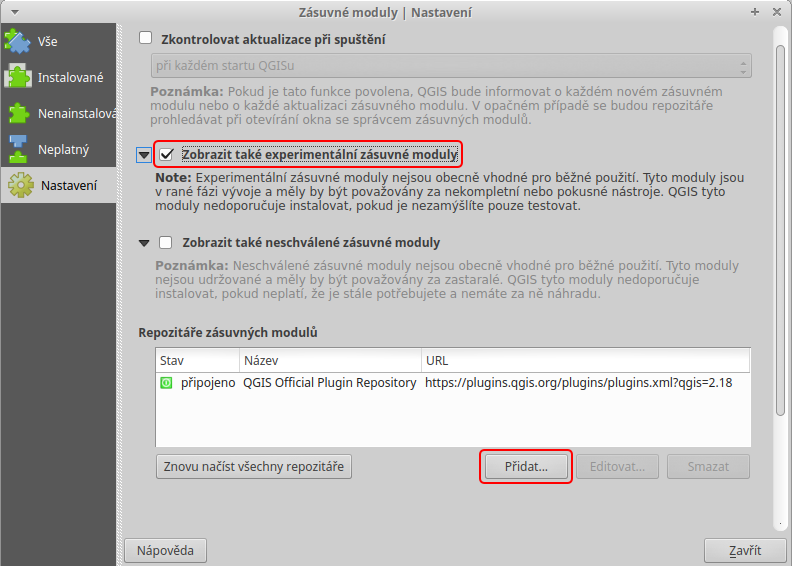
\includegraphics[width=.9\textwidth]{./pictures/pridani_repozitare.png}
		\caption[Přidání repozitáře]{Přidání repozitáře}
		\label{fig:pridani_repozitare}
 	\end{figure}
 	
	\begin{figure}[H]
		\centering
		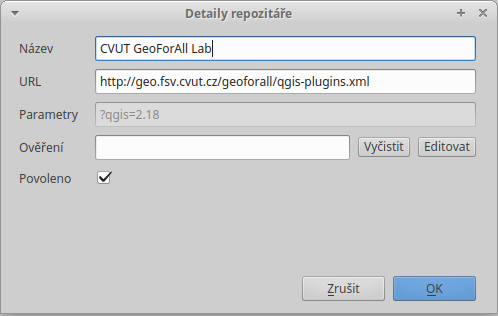
\includegraphics[width=.6\textwidth]{./pictures/pridani_repozitare-geoforall_lab.png}
		\caption[Přidání repozitáře GeoForAll Lab]{Přidání repozitáře GeoForAll Lab}
		\label{fig:pridani_repozitare_geoforall_lab}
 	\end{figure}

	\begin{figure}[H]
		\centering
		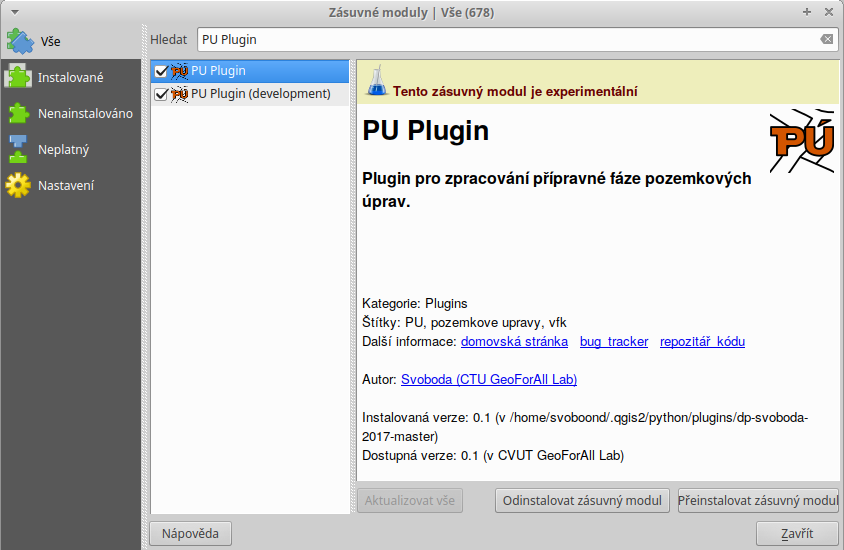
\includegraphics[width=.8\textwidth]{./pictures/instalace_puplugin.png}
		\caption[Instalace zásuvného modulu]{Instalace zásuvného modulu}
		\label{fig:instalace_puplugin}
 	\end{figure}

Když je plugin nainstalován, objeví se v~liště zásuvných modulů jeho ikona (viz obr.~\ref{fig:ikona_puplugin}). Okno zásuvného modulu je možné vyvolat poklepáním na~jeho ikonu nebo volbou \textit{Zásuvné moduly $\rightarrow$ PU Plugin $\rightarrow$ PU Plugin}.

	\begin{figure}[H]
		\centering
		
\includegraphics[width=.1\textwidth]{./pictures/puplugin.png}
		\caption[Ikona zásuvného modulu]{Ikona zásuvného modulu}
		\label{fig:ikona_puplugin}
 	\end{figure}